\documentclass{article}
\usepackage{graphicx}
\usepackage{placeins} % Required for inserting images
\setlength\parindent{0pt}
\title{DL-Exercise 1}
\author{th273, mg776, kb301}
\date{October 2023}

\begin{document}

\maketitle

\section{Eigendecomposition}
Card 1: Black-Black - BB
\\
Card 2: White-White - WW
\\
Card 3: Black-White - BW
\\\\
$$P(BB)=P(WW)=P(BW)=\frac{1}{3}$$
\\\\
\\
\subsection{What are the probabilities that the card on the table shows a black side? What are the probabilities it shows a white side?}
$$P(see Black)=1\cdot\frac{1}{3}+0\cdot\frac{1}{3}+\frac{1}{3}\cdot\frac{1}{2}=\frac{2}{6}+\frac{1}{6}=\frac{1}{2}$$
\\\\
$$P(see White)=\frac{1}{2}$$
\subsection{If we draw a card and it shows black, compute the probability that the other side of the card is also black.}
Too see Black on the second time we needed to draw Card 1- BB
\\\\
$$P(see Black|BB) = 1$$ The Probability to see black on the first time given we have drawn card 1(BB) is obviously 100\%
\\\\
$$P(BB| see Black)=\frac{P(see Black|BB) P(BB)}{P(see Black)}=\frac{1\cdot\frac{1}{3}}{\frac{1}{2}}=\frac{2}{3}$$
\subsection{Find the probability that the other side of the card is black if the card shows a white side.}
Too see white on the first and black on the second time we needed to draw Card 3- BW
\\\\
$$P(see white|BW) = \frac{1}{2}$$ The Probability to see white on the first time given we have drawn card 3(BW) is obviously 50\%
\\\\
$$P(BW| see white)=\frac{P(see white|BW) P(BW)}{P(see white)}=\frac{\frac{1}{2}\cdot\frac{1}{3}}{\frac{1}{2}}=\frac{2}{6}=\frac{1}{3}$$
\pagebreak
\section{Distributions and Central Limit Theorem}
\subsection{Central Limit Theorem}
As depicted in figure \ref{fig:clt}, the approximation increases in precision with growing
sample sizes.
With sample size 1, it is the original distribution.
With 1024 samples, both match the normal distribution.
    \begin{figure}[H]
        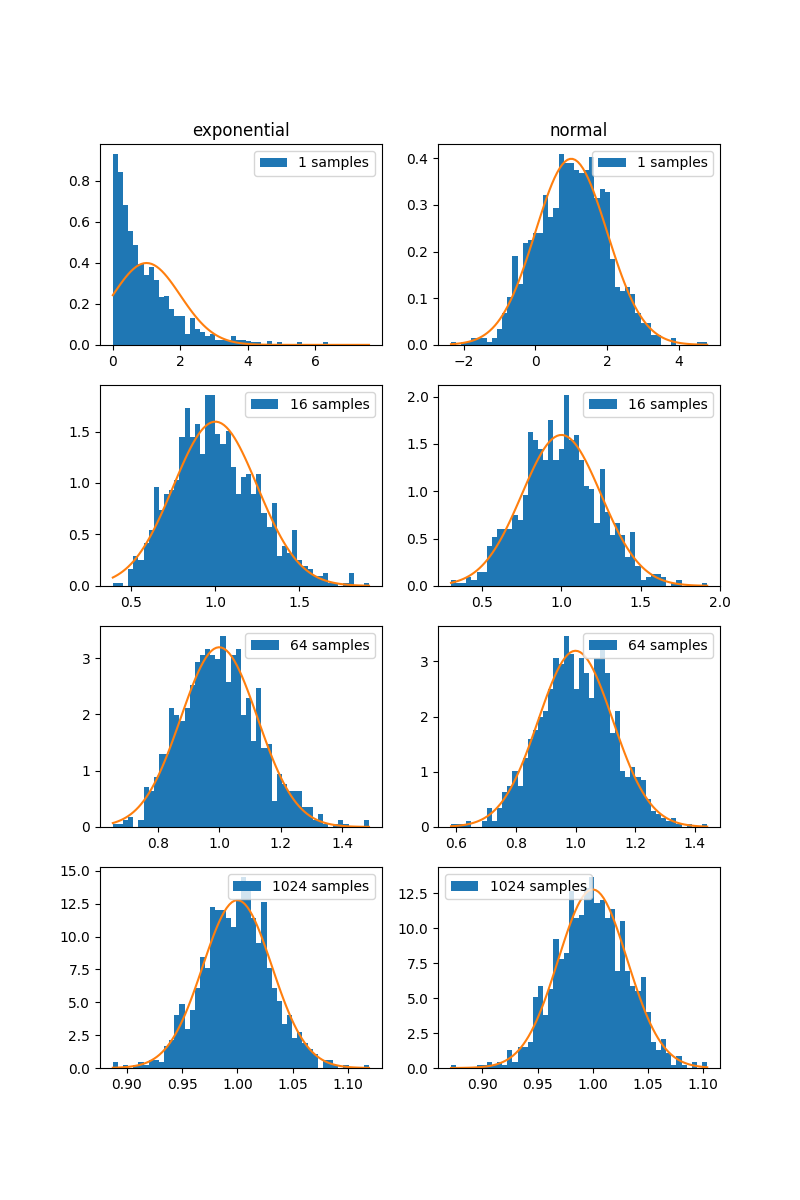
\includegraphics[width=\textwidth]{clt.png}
        \caption{Plot of the Central limit theorem code.}\label{fig:clt}
    \end{figure}
\FloatBarrier

\subsection{Bayesian Linear Regression}
In figure \ref{fig:2D}, the prior and posterior gaussian distributions are visualized.
As expected, the posterior is more certain than the prior, with lower variance and higher bias.
    \begin{figure}[H]
        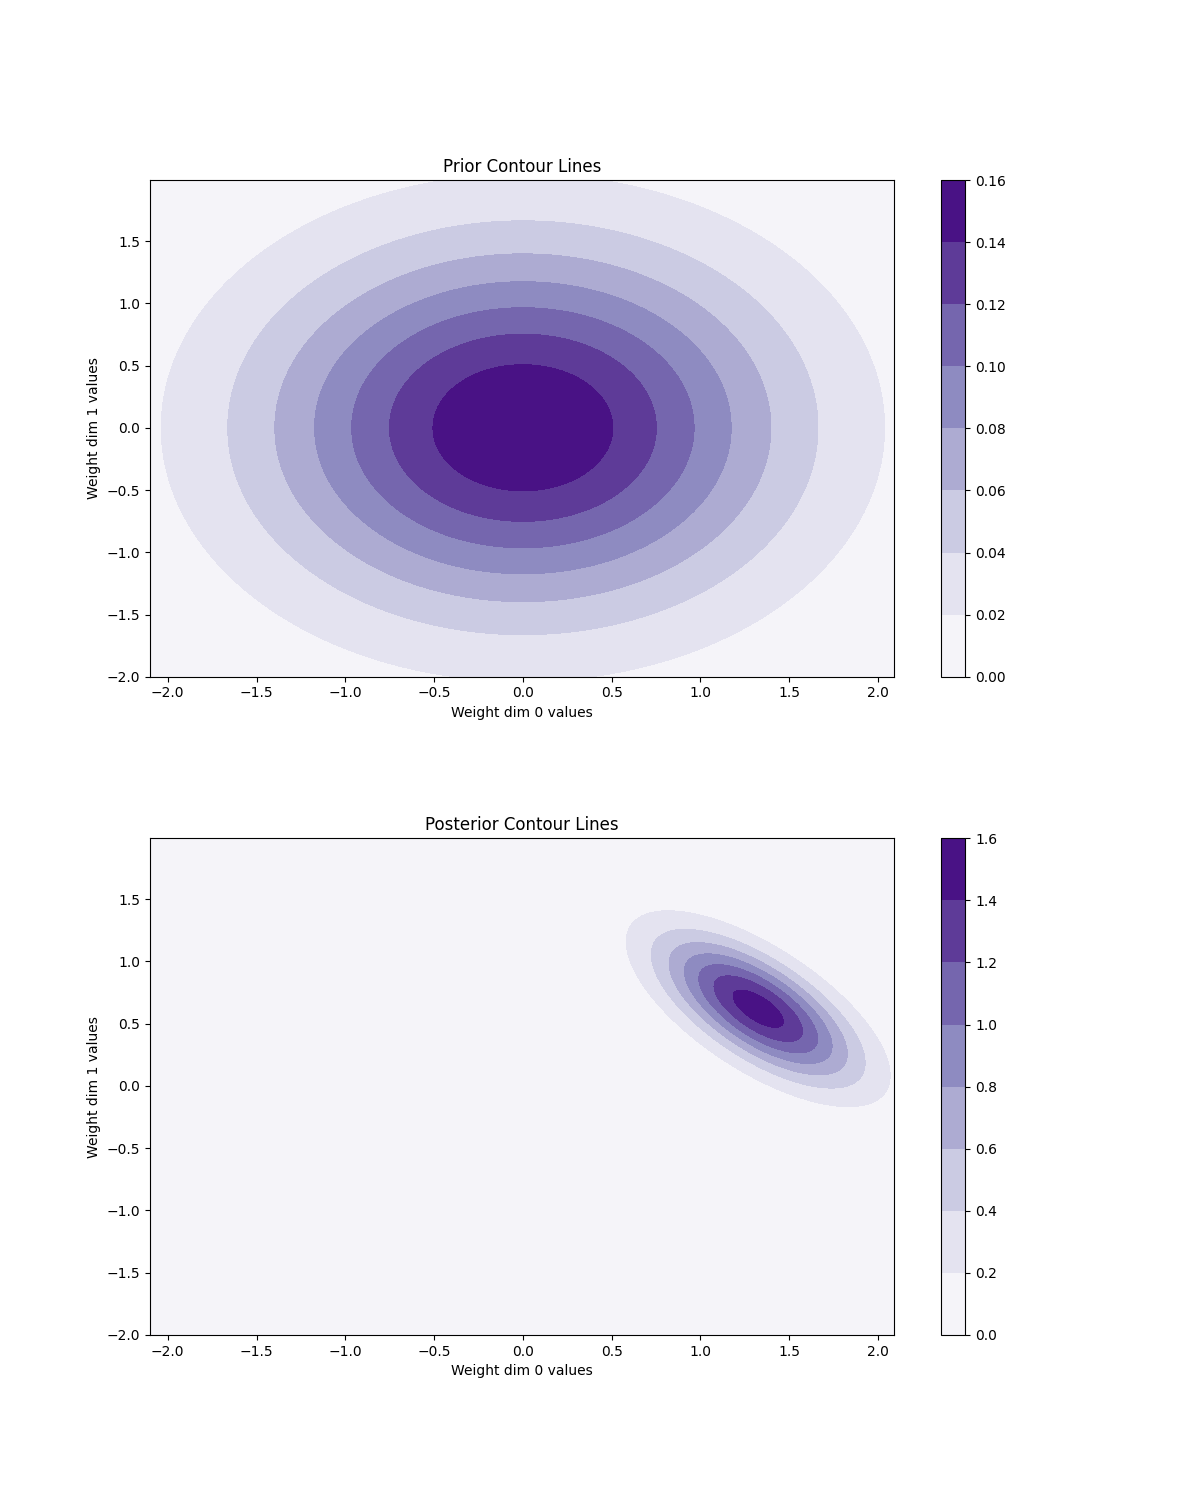
\includegraphics[width=\textwidth]{2D_distr.png}
        \caption{Plot of the prior and posterior gaussian distributions.}\label{fig:2D}
    \end{figure}
\end{document}
